\vspace{-3cm}\chapter{实验4. 模式化打印图形}

\section{4.1 题目}

编写一个程序,通过命令行参数的方式,接收两个参数。参数1指定打印的图形模式(分别为下图中的
$a\backslash b\backslash c\backslash d\backslash e$),
参数2指定打印的图形的大小(一个非负整数),下面的模式图以大小\textbf{7}为例进行展示:

\begin{figure}[H]
    \centering
    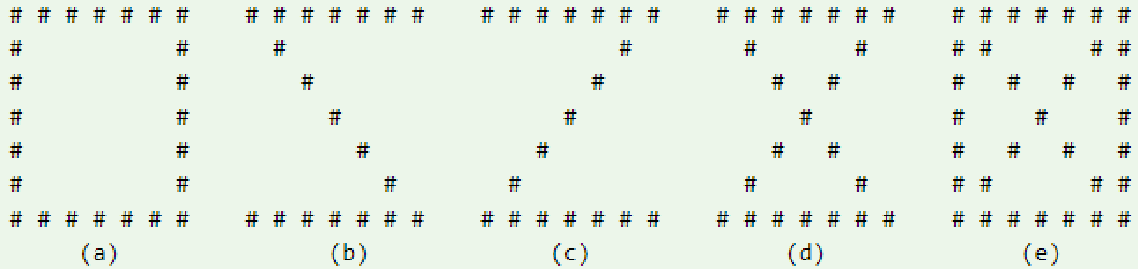
\includegraphics[width = 0.8\textwidth]{../pic/4/4.0.png}
\end{figure}

\section{4.2 思路分析}

\begin{enumerate}
    \item \textbf{数据输入}. 数据以String的形式从命令行输入
    \item \textbf{程序思路}.
    \begin{itemize}
        \item 可以把打印部分作为一个矩阵,如果矩阵中的某个元素行和列满足某种规律则打印\lstinline{#},否则打印\text{ }(空格).
            通过观察可知,矩阵大小为\lstinline{[n][2n-1]}. 我们可以不必真的开一个\lstinline{int}或\lstinline{boolean}二维数组的变量,
            而是直接打印出来。
        \item 题目就提示这道题的思路,模块化打印: 分别对五种模式写五种打印函数,对输入的第一个参数\lstinline{switch}. 
            \begin{itemize}
                \item[a.] 第0列和第n-1列所有元素,第0行和第n-1行偶数索引的元素
                \item[b.] 行数等于列数/2,第0行,第n-行的偶数索引的元素
                \item[c.] 行数等于列数/2,第0行,第n-行的偶数索引的元素
                \item[d.] b和c的结合
                \item[e.] a和d的结合
            \end{itemize}
        \item 虽然五种模式的打印有一定的交叉,甚至可以通过两个叠加得到第三个,但如果只实现其中的几个函数意味着要对整个矩阵块扫描两次,
            而且要存储其状态,原先的思路是直接打印不存储。
    \item \textbf{数据测试}. 打印图像题,采用题目数据通过即可。
    \end{itemize}
\end{enumerate}

\section{4.3 代码与结果}

4.2中程序思路已经说的很清楚,代码中存在较多重复的,不再列出,具体附于附录。

运行结果如下

\begin{figure}[H]
    \centering
	\begin{subfigure}{0.19\linewidth}
		\centering
		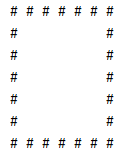
\includegraphics[width=1\linewidth]{../pic/4/4.a.png}
        \caption{input: a 7}
	\end{subfigure}
	\begin{subfigure}{0.19\linewidth}
		\centering
		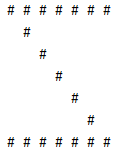
\includegraphics[width=1\linewidth]{../pic/4/4.b.png}
        \caption{input: b 7}
	\end{subfigure}
	\begin{subfigure}{0.19\linewidth}
		\centering
		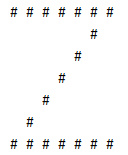
\includegraphics[width=1\linewidth]{../pic/4/4.c.png}
        \caption{input: c 7}
	\end{subfigure}
    \begin{subfigure}{0.19\linewidth}
		\centering
		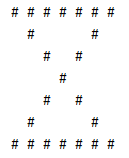
\includegraphics[width = 1\linewidth]{../pic/4/4.d.png}
        \caption{input: d 7}
	\end{subfigure}
	\begin{subfigure}{0.19\linewidth}
		\centering
		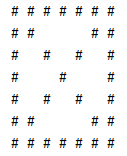
\includegraphics[width=1\linewidth]{../pic/4/4.e.png}
        \caption{input: e 7}
	\end{subfigure}
    \caption{Output of Problem4}
\end{figure}

\section{4.4 总结与收获}

本题较为简单,但一开始输出时我以为矩阵是\lstinline{[2n-1][2n-1]},测试时才注意到,以后读题一定要更仔细一点,
不要再因为这种间距不同导致理解产产生问题